In this chapter planning and work-flow regarding Sprint 3 will be described. 
All from setting our goals to implementation and testing. On the end we will evaluate whole sprint and try to answer on following questions: What went well? What could be improved? What should we start doing?  
% TODO rewrite

\section{Sprint planning}
In the planning part of sprint 2 when there have been introduced and idea or goal for refining and extent the existing code, customer agreed, with condition, that sprint 3 will be focused on image processing part.

As the image processing module was one of the major risks there was done some preliminary studies research even in sprint 2 about possible approaches.
One specific way to deal with the problem was introduced to customer in planning part of meeting.
Customer was not satisfied with such a low-level approach and wanted us to use some existing tools.
Therefore there was need for additional preliminary studies concerning existing projects or libraries that could be used.
You can read more about additional preliminary studies below.

This time there was made an offer of additional "pre-demo" video showing the progress of implementation on Thursday 4.10.2013 during our regular meeting and customer gladly accepted this proposal.


\begin{figure}[H]
	\centering
		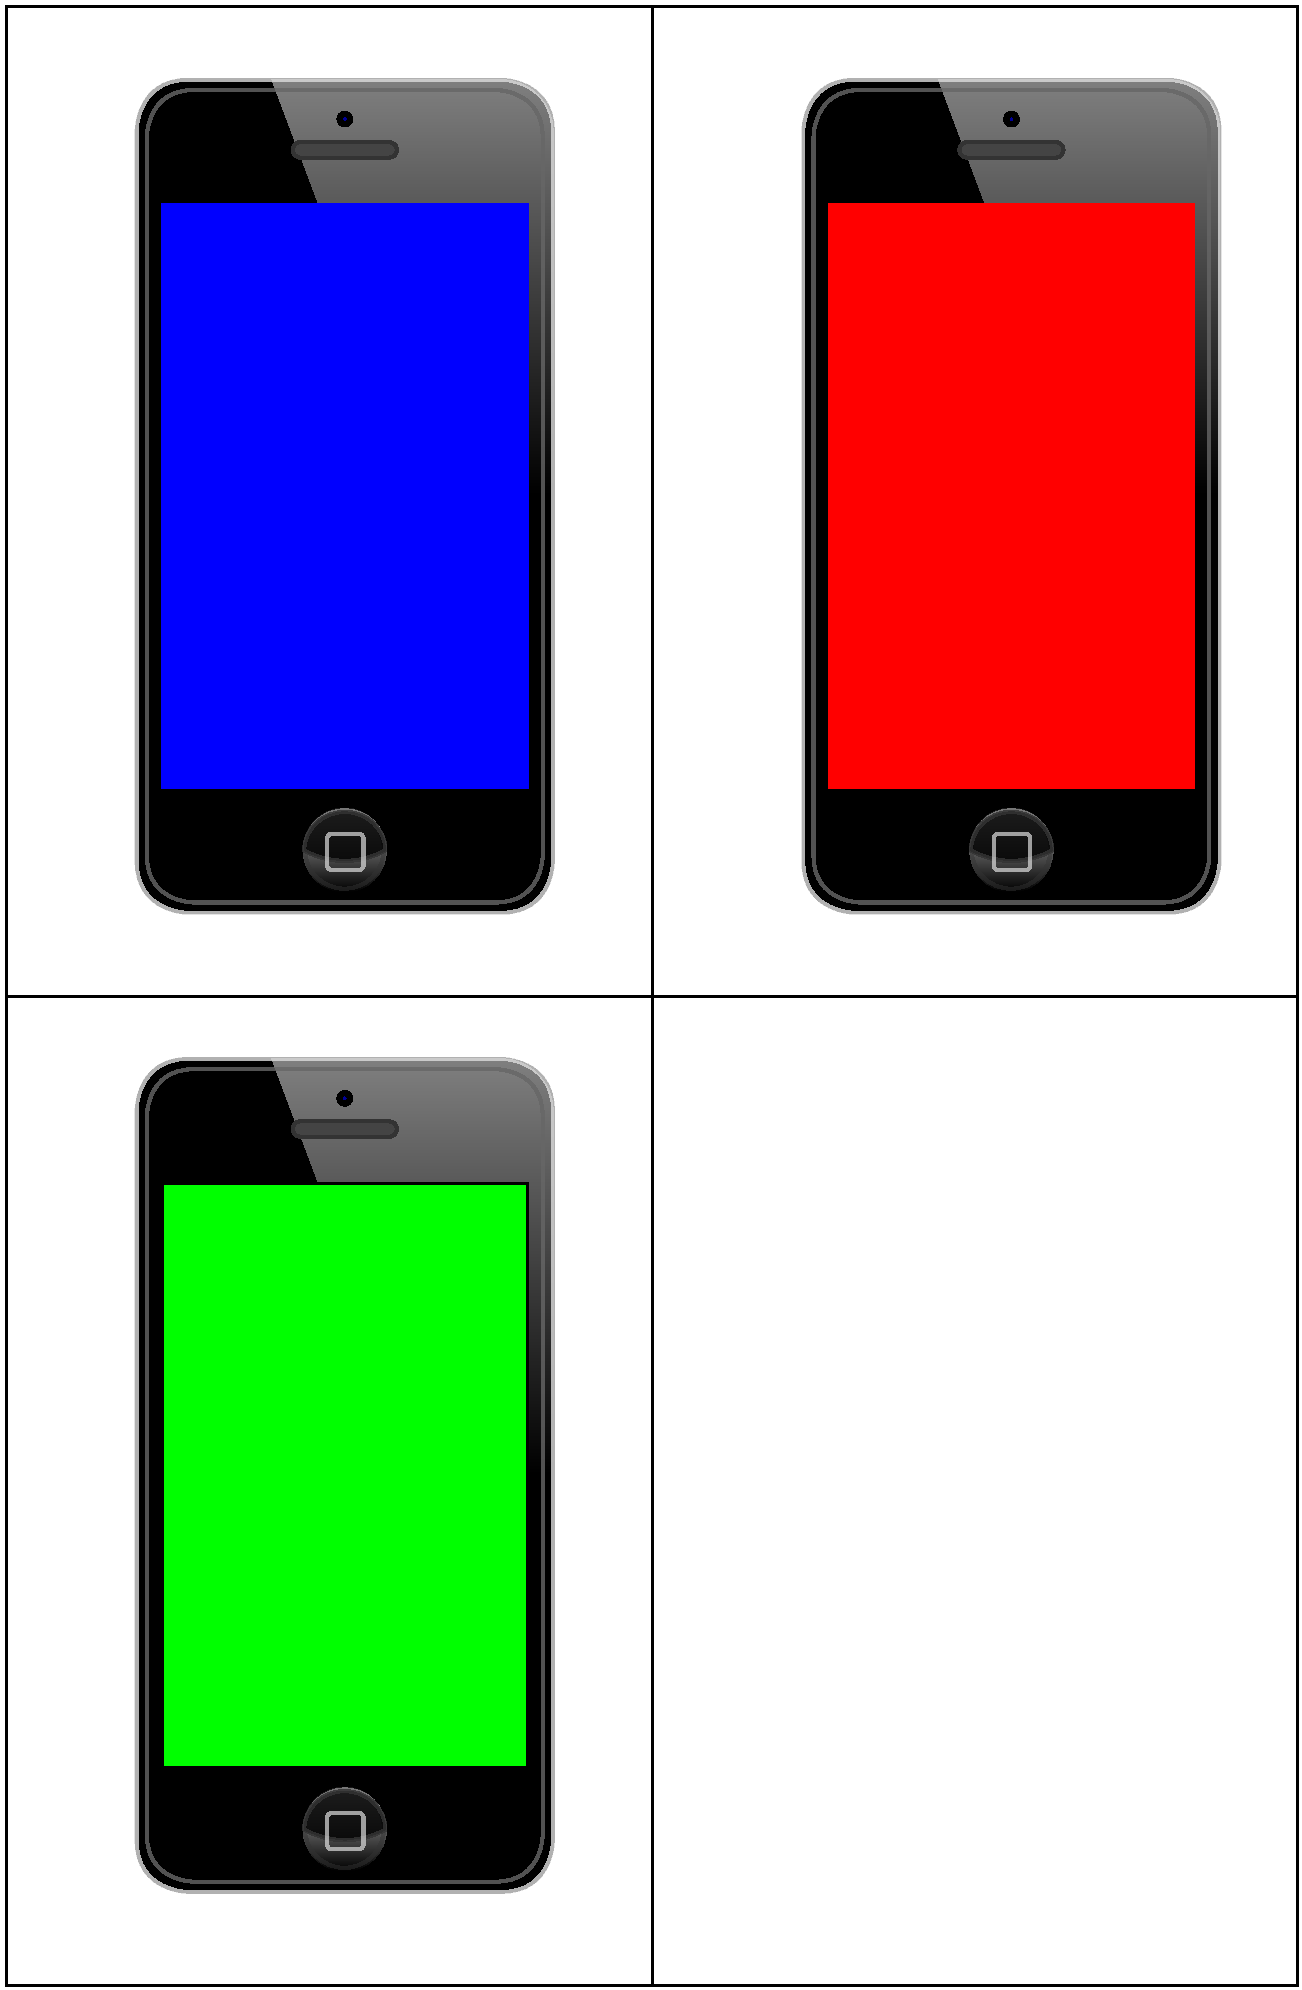
\includegraphics[width=7cm]{sprint3/sprint3_goal.pdf}
	\caption{Example of ideal data input for image processing module with 2x2 matrix.}
	\label{img:sprint3_goal}
\end{figure}

\subsection{Duration}
This sprint will be 2 weeks long. From 30.09.2013 to 13.10.2013.
We agreed on the date of presentation and showing the running demo -- Thursday 11.10.2013.
Estimated velocity is 240h since we agreed on 30 working hours per person per week.

\subsection{User-stories}

\subsubsection*{Implementation}
All the functional requirements for sprint 3 are presented in table \ref{tab:sprint3stories}
\LTXtable{\textwidth}{sprint3/stories.tex}

\subsubsection*{Documentation}
All the documentation stories for sprint 3 are presented in table \ref{tab:sprint3Documentationstories}
\LTXtable{\textwidth}{sprint3/storiesDocumentation.tex}

\subsubsection*{Process}
All the Process stories for sprint 3 are presented in table \ref{tab:sprint3storiesProcess}
\LTXtable{\textwidth}{sprint3/storiesProcess.tex}

\section{Sprint goal}
The goal of this sprint is having a working application on a mobile phone that can work in two modes.  
Input type and output are for both modes common -- input is an image or video and output is location of detected mobile phones in a given matrix (e.g. 4x4 matrix) with color that mobile's screen is lighting.
In the first mode, real video from mobile's camera will be treated as an input and on the other hand in the second mode mock data (image/video) are treated as an input.

You can see example of input with matrix 2x2 in image. Appropriate output of image processing and mapping module will be: \texttt{\{blue,[0,0]\}, \{red,[1,0]\}, \{green,[0,1]\}}.
\section{Preliminary studies}
% TODO

\section{System Burndown}
\section{Architecture}
In this section will be described image processing module using 4+1 architectural view module.

\subsection{Logical view}

\begin{figure}[H]
	\centering
		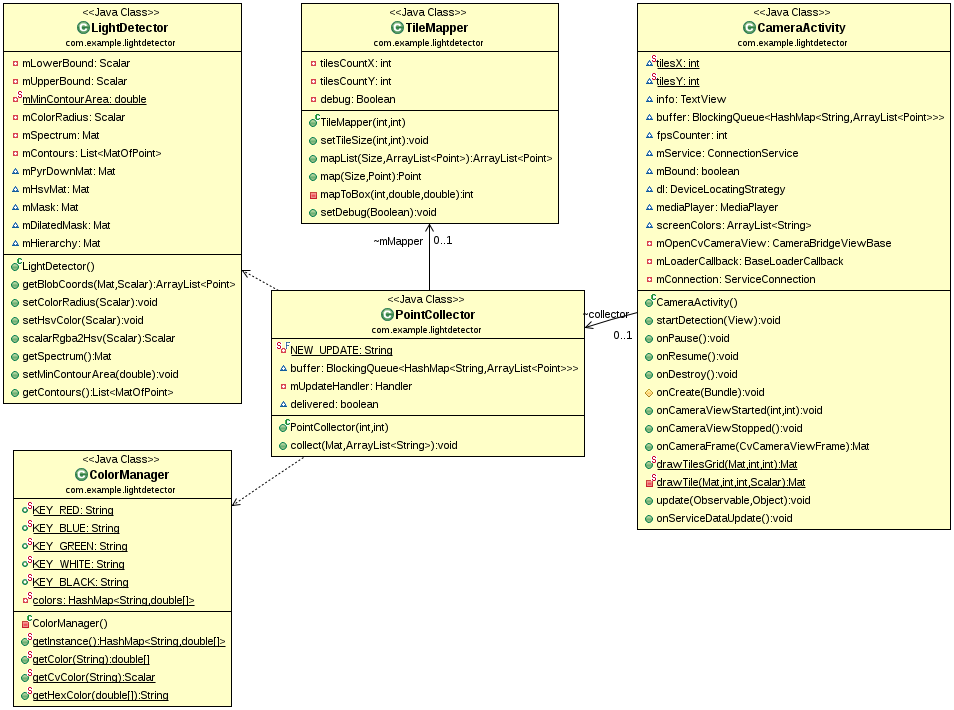
\includegraphics[width=10cm]{sprint3/sprint3.png}
	\caption{Sprint 3 light detection module class diagram}
	\label{fig:class_diagram_sprint3}
\end{figure}

\subsection{Physical view}
\subsection{Process view}
\subsection{Development view}

\section{Implementation}


\section{Testing}


\section{Occurring risks}
\section{Retrospective}
\subsection{Pros}
\subsection{Cons}
\section{Evaluation}